\documentclass[11pt,xcolor={dvipsnames},usepdftitle=false]{beamer}
%\usepackage{presentation}
\usepackage{tikz}
\usetikzlibrary{positioning,arrows.meta,shapes,decorations,calc,fit}

%\hypersetup{pdftitle={Section 4: Regression and Omitted Variable Bias}}

% TikZ settings for DAGs
\tikzset{
    -Latex,auto,node distance=1cm and 1cm,semithick,
    state/.style={ellipse, draw, minimum width=0.7cm},
    point/.style={circle, draw, inner sep=0.04cm,fill,node contents={}},
    bidirected/.style={Latex-Latex},
    el/.style={inner sep=2pt, align=left}
}

% Custom commands
\newcommand{\indep}{{\bot\negthickspace\negthickspace\bot}}

\begin{document}

\title{Causal Inference}
%\information{}{Section 4: Regression and Omitted Variable Bias}

\frame{\titlepage}

%--------------------------------------
\begin{frame}
\frametitle{Omitted variable bias}
\begin{itemize}
\item Regression gives us a description of the CEF, but CEF only gives us a causal relationship if all backdoor paths are closed by conditioning
\item In practice, hard to know if our set of controls includes all relevant confounding variables
\end{itemize}

\begin{center}
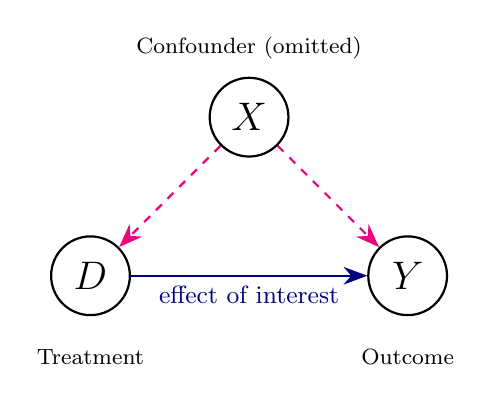
\begin{tikzpicture}[
    node distance=2.5cm and 3cm,
    >={Stealth[length=3mm]},
    varnode/.style={circle, draw=black, thick, minimum size=1cm, font=\Large},
    causal/.style={->, thick, NavyBlue},
    confound/.style={->, thick, RubineRed, dashed}
]

% Nodes
\node[varnode] (D) {$D$};
\node[varnode, right=of D] (Y) {$Y$};
\node[varnode, above=1.5cm of $(D)!0.5!(Y)$] (X) {$X$};

% Edges
\draw[causal] (D) -- node[below, font=\small] {effect of interest} (Y);
\draw[confound] (X) -- node[left, font=\small, align=right] {} (D);
\draw[confound] (X) -- node[right, font=\small, align=left] {} (Y);

% Labels
\node[below=0.3cm of D, font=\footnotesize] {Treatment};
\node[below=0.3cm of Y, font=\footnotesize] {Outcome};
\node[above=0.1cm of X, font=\footnotesize] {Confounder (omitted)};

\end{tikzpicture}
\end{center}
\end{frame}

%--------------------------------------
\begin{frame}
\frametitle{Reasoning about bias}
\begin{itemize}
\item DAGs are yes-no propositions: did you condition correctly?
\item In practice, answer is likely `probably?', not `yes'/`no'
\item Going to make the meaning of `probably' precise by asking: \al{How sensitive is our estimate of the causal effect to an unobserved confounder?}
\item Ingredients for this:
\begin{itemize}
    \item A statistical model summarizing the relationship between treatment, potential confounders, and outcome
    \item A deeper understanding of the mechanics of that model
    \item \al{Real-world knowledge} about the relative strength of observed and unobserved confounders
\end{itemize}
\end{itemize}
\end{frame}

%--------------------------------------
\begin{frame}
\frametitle{Omitted variable bias in a regression}
\begin{itemize}
\item The model we want is: $ Y_i = \color{NavyBlue}{\alpha + \rho D_i + \theta X_i + e_i}$
\item But we only have: $ Y_i = \lambda + \beta D_i  + u_i $

\item How does leaving out $X_i$ bias our estimated $\beta$, $\frac{Cov(Y_i,D_i)}{Var(D_i)}$?

{\small
\begin{align*}
Cov(Y_i,D_i)
  &= Cov(\textcolor{NavyBlue}{\alpha + \rho D_i + \theta X_i + e_i}, D_i) \\
  &= Cov(\alpha,D_i) + Cov(\rho D_i, D_i) + Cov(\theta X_i , D_i) + Cov(e_i,D_i) \\
  &= \rho \, Cov(D_i, D_i) + Cov(\alpha,D_i) + Cov(\theta X_i , D_i) \\
  &= \rho \, Var(D_i) + \theta Cov(X_i , D_i)
\end{align*}}

\[
\frac{Cov(Y_i,D_i)}{Var(D_i)}
  = \rho + \theta \times \underbrace{\frac{Cov( X_i , D_i)}{Var(D_i)}}_{\text{What is this?}} = \rho + \underbrace{\delta}_{impact} \times \underbrace{\gamma}_{imbalance}
\]
\end{itemize}
\end{frame}

%--------------------------------------
\begin{frame}
\frametitle{Omitted variable bias (continued)}
\begin{itemize}
\item Same holds if we include other covariates $Z$ in the observed model and think of $\delta$ and $\gamma$ as regression coefficients after residualizing wrt $Z$
\item For imbalance:
\begin{itemize}
    \item Take the leftover variation of our unobserved confounder after taking out the linear relationship with $Z$.
    \item Then ask: what is the strength of the relationship between that confounder and the treatment
\end{itemize}

\end{itemize}

\[
\frac{Cov(\tilde{Y_i},\tilde{D_i})}{Var\tilde{(D_i)}}
  = \rho + \underbrace{\tilde{\delta}}_{impact} \times \underbrace{\tilde{\gamma}}_{imbalance}
\]
\end{frame}

%--------------------------------------
\begin{frame}
\frametitle{Thinking about confounding in terms of $R^2$}
\[R^2 = \frac{Var(\hat{Y})}{Var(Y)} = corr(Y, \hat{Y} )^2\]

\begin{itemize}
\item $R^2$ measures the proportion of variance in the outcome explained by variance in the predicted outcome from the regression
\item Positive characteristics: not dependent on scale of outcome
\item Negative characteristics: you can always increase $R^2$ by putting more variables into your regression
\item We can express OVB in terms of partial $R^2$
\[|\tilde \delta \times  \tilde \gamma |
= \widehat{\text{se}}(\rho)
  \sqrt{
    \frac{
      R^2_{Y \sim Z \mid D, X} \;
      R^2_{D \sim Z \mid X}
    }{
      1 - R^2_{D \sim Z \mid X}
    }
  }
  \; (\text{df}).
\]
\end{itemize}
\end{frame}

%--------------------------------------
\begin{frame}
\frametitle{Thinking about confounding in terms of $R^2$}
\begin{itemize}
\item How do we think about each term here intuitively? Which ones can we benchmark against observed confounders?
\[|\tilde \delta \times  \tilde \gamma |
= \widehat{\text{se}}(\rho)
  \sqrt{
    \frac{
      R^2_{Y \sim Z \mid D, X} \;
      R^2_{D \sim Z \mid X}
    }{
      1 - R^2_{D \sim Z \mid X}
    }
  }
  \; (\text{df}).
\]
\item Some questions:
\begin{itemize}
\item What increases and decreases bias?
\item What happens to $R^2_{Y \sim Z \mid D, X}$ as I include more control variables in my regression?
\end{itemize}
\end{itemize}
\end{frame}

%--------------------------------------
\begin{frame}
\centering
\heading{Application: Sensitivity Analysis}
\end{frame}

%--------------------------------------
\begin{frame}
\frametitle{Example: Support for the radical right in German elections}
Starting in the 2010s, vote shares for radical right-wing parties have been increasing across Europe. The change has been most pronounced in rural areas.
\begin{itemize}
    \item \al{Research Question:}
    \item Does membership in a community that was historically been peripheral to the nation state cause modern individuals to vote for radical right parties?
\end{itemize}
\end{frame}

%--------------------------------------
\begin{frame}
\frametitle{Regression controls}
Country-level:\\
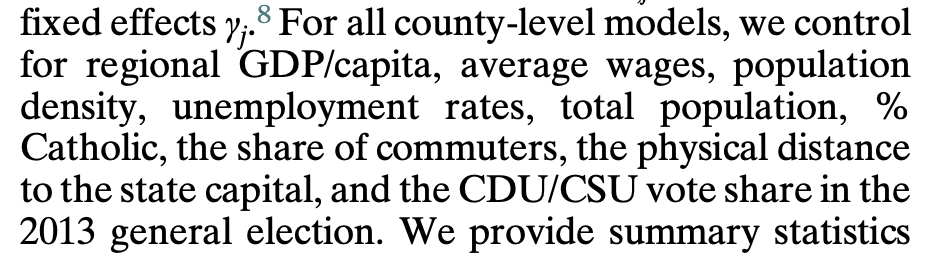
\includegraphics[width=.8\textwidth]{images/ziblatt_controls-1.png}
\vspace{3mm}

Individual-level:\\
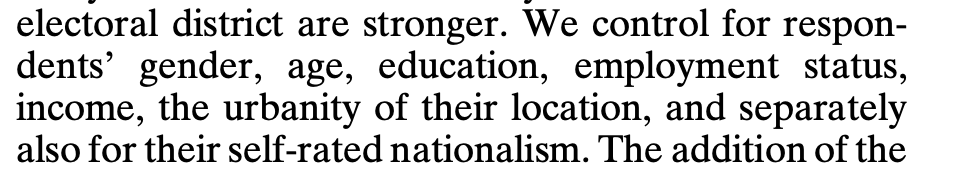
\includegraphics[width=.8\textwidth]{images/ziblatt_controls-2.png}
\end{frame}

%--------------------------------------
\begin{frame}
\frametitle{Sensitivity analysis results}
\begin{center}
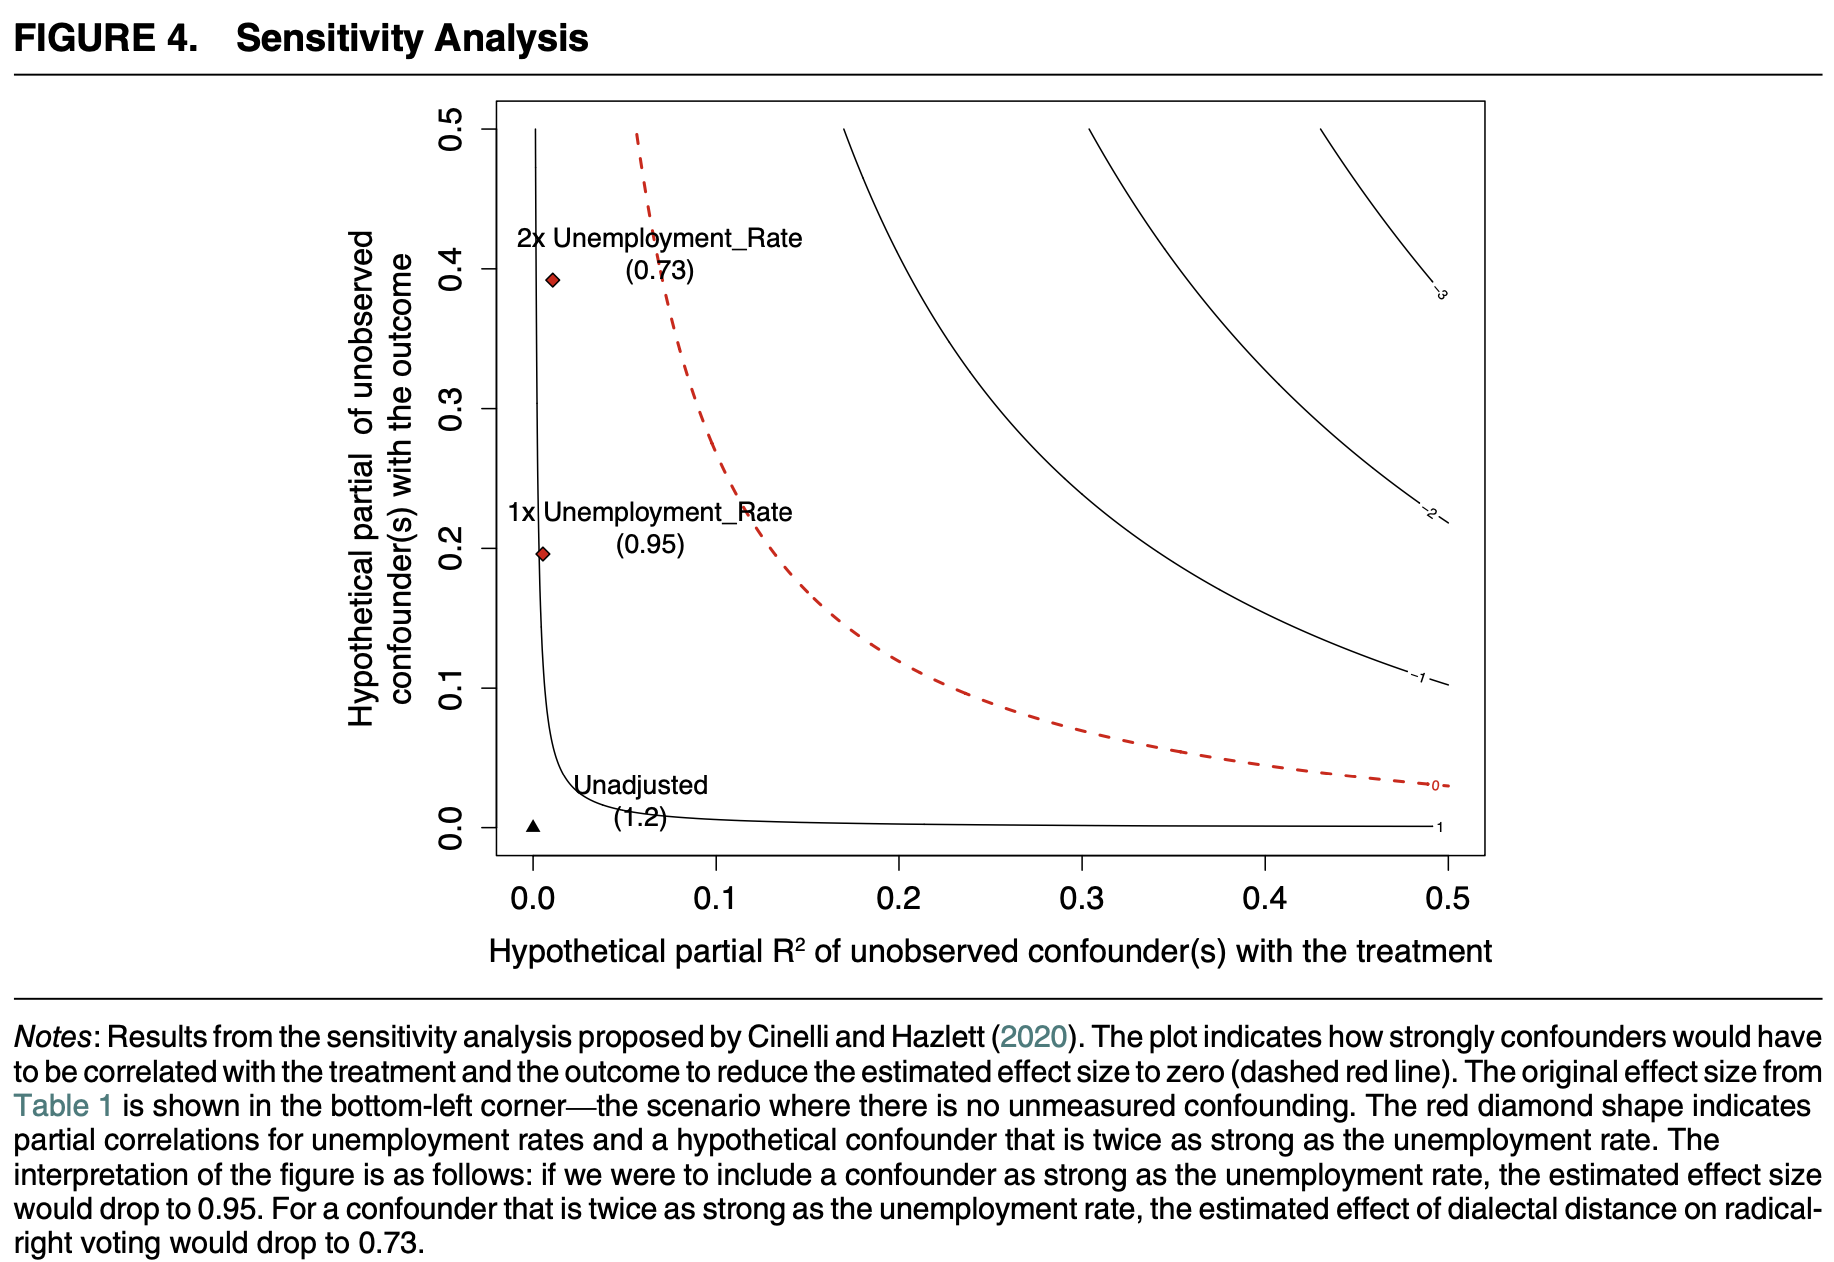
\includegraphics[width=\textwidth]{images/ziblatt_ovb.png}
\end{center}
\end{frame}

%--------------------------------------
\lastslide

\end{document}
